\chapter{Étude de l'asservissement de la MCC}

\section{Asservissement en courant}

L'asservissement en courant du moteur constitue la boucle interne de notre système de régulation en cascade. Son rôle principal est d'assurer que le courant absorbé par le moteur suive fidèlement la consigne fournie par l'asservissement en vitesse. Cette régulation permet de contrôler précisément le couple moteur et d'améliorer la dynamique globale du système.

\subsection{Modélisation sur Simulink}

L'asservissement en courant doit appliquer la consigne déterminée par l'asservissement en vitesse. Pour cela, nous mettons en œuvre un correcteur Proportionnel-Intégral (PI). Le cahier des charges impose un temps de réponse égal à 10 fois la période de la modulation de largeur d'impulsion (MLI), soit \SI{0,45}{ms}, avec un dépassement maximal de \SI{20}{\percent}.

À l'aide de l'outil PID Tuner de Simulink, nous obtenons les paramètres optimaux suivants pour le correcteur PI :
\begin{itemize}
    \item Gain proportionnel : $K_p = 5,053$
    \item Gain intégral : $K_i = 36\,349,55$
\end{itemize}

Il est important de souligner que la notation du correcteur PI diffère entre Simulink et PSIM. Sur PSIM, la valeur du paramètre $\tau$ représente le rapport $\dfrac{K_p}{K_i}$, tandis que sur Simulink, les deux gains sont exprimés directement.

% image de l'asservissement en courant Simulink
\begin{figure}[H]
    \centering
    \includegraphics[width=1\textwidth]{images/BF_Courant/Schéma_Simulink_Asservissement_Courant.png}
    \caption{Schéma de l'asservissement en courant du moteur dans Simulink}
    \label{fig:asservissement_courant_simulink}
\end{figure}
\figref{Figure \ref{fig:asservissement_courant_simulink}}{Modélisation\_Intermédiaire\_VALIDE/03\_BF\_Courant/BF\_Courant\_VALIDE\_06\_11\_2025.slx}

\subsection{Modélisation sur PSIM}

Pour adapter le correcteur PI de Simulink à PSIM, il faut convertir les paramètres en utilisant les relations suivantes :

Dans Simulink : 
\[ G(s) = K_p + \dfrac{K_i}{s} = K_p \dfrac{s + \tfrac{K_i}{K_p}}{s} \]

Dans PSIM : 
\[ G(s) = k \dfrac{1 + sT}{sT} \Rightarrow k = K_p \text{ et } T = \dfrac{K_p}{K_i} \]

\newpage
% image de l'asservissement en courant PSIM
\begin{figure}[H]
    \centering
    \includegraphics[width=1\textwidth]{images/BF_Courant/Schéma_PSIM_Asservissement_Courant.png}
    \caption{Schéma de l'asservissement en courant du moteur dans PSIM}
    \label{fig:asservissement_courant_psim}
\end{figure}
\figref{Figure \ref{fig:asservissement_courant_psim}}{Modélisation\_Intermédiaire\_VALIDE/03\_BF\_Courant/BF\_Courant\_VALIDE\_06\_11\_2025.psimsch}


\subsection{Comparaison des résultats}

Dans cette section, nous allons comparer les résultats obtenus avec les deux outils de simulation, Simulink et PSIM.

% image de la comparaison des réponses
\begin{figure}[H]
    \centering
    \includegraphics[width=1\textwidth]{images/BF_Courant/Courbe_Comparaison_Asservissement_Courant.png}
    \caption{Comparaison des réponses indicielle de l'asservissement en courant du moteur entre Simulink et PSIM}
    \label{fig:comparaison_reponse_indicielle_courant}
\end{figure}
\figref{Figure \ref{fig:comparaison_reponse_indicielle_courant}}{Modélisation\_Intermédiaire\_VALIDE/03\_BF\_Courant/Comparaison\_Asservissement\_Courant\_VALIDE\_06\_11\_2025.m}

La figure \ref{fig:comparaison_reponse_indicielle_courant} illustre la comparaison des réponses indicielle de l'asservissement en courant du moteur entre Simulink et PSIM. Les deux courbes sont quasiment superposées, ce qui confirme la cohérence des modélisations réalisées dans les deux environnements.

On constate que la réponse indicielle de l'asservissement en courant du moteur présente un dépassement d'environ 19\% et un temps de réponse de 0,35 ms. Ce qui respecte les spécifications du cahier des charges qui exige un dépassement maximal de 20\% et un temps de réponse maximal de 10 fois la prériode de la MLI soit 0,45 ms.

\newpage
\section{Asservissement en vitesse}

L'asservissement en vitesse constitue la boucle externe et la régulation principale de notre système de contrôle en cascade. Contrairement à l'asservissement en courant qui opère sur une grandeur électrique interne, l'asservissement en vitesse agit directement sur la grandeur mécanique d'intérêt pour l'application finale. C'est donc cet asservissement qui détermine les performances réelles du système vis-à-vis des exigences du cahier des charges.

La régulation en vitesse permet de garantir que le moteur atteint et maintient la vitesse de rotation souhaitée, indépendamment des perturbations externes telles que les variations de charge ou les frottements. Elle assure également la rapidité de la réponse du système face aux changements de consigne, tout en limitant les dépassements pour éviter les sollicitations mécaniques excessives.

Dans cette section, nous allons d'abord caractériser le comportement du système en boucle ouverte pour identifier ses limitations, puis nous concevrons un correcteur PI permettant d'améliorer significativement les performances dynamiques du moteur.

\subsection{Caractérisation en boucle ouverte}

Nous commençons par la simulation de la vitesse du moteur en boucle ouverte sur Simulink afin d'établir une référence de performance. Nous réalisons le schéma suivant :

\begin{figure}[H]
    \centering
    \includegraphics[width=1\textwidth]{images/BO_Vitesse/Schéma_Simulink_BO_Vitesse.png}
    \caption{Schéma de la simulation en boucle ouverte de la vitesse du moteur dans Simulink}
    \label{fig:schéma_BO_vitesse_simulink}
\end{figure}
\figref{Figure \ref{fig:schéma_BO_vitesse_simulink}}{Modélisation\_Intermédiaire\_VALIDE/04\_BF\_Courant\_Vitesse/BO\_Vitesse/BO\_Vitesse\_VALIDE\_06\_11\_2025.slx}

La simulation en boucle ouverte nous permet d'observer la réponse naturelle du système sans rétroaction. Cette étape est essentielle pour comprendre les limites intrinsèques du système et établir les objectifs d'amélioration pour l'asservissement. Pour effectuer cette caractérisation, nous attendons d'abord que le système atteigne son régime permanent, puis nous appliquons une consigne en échelon pour observer la dynamique de réponse.
\vspace{0.5cm}

L'analyse de la réponse indicielle révèle un temps de réponse à \SI{5}{\percent} en boucle ouverte de \SI{124,1}{ms}. Cette valeur relativement élevée indique une dynamique lente qui ne serait pas acceptable pour de nombreuses applications industrielles nécessitant des temps de réaction rapides.

\newpage
\begin{figure}[H]
    \centering
    \includegraphics[width=0.8\textwidth]{images/BO_Vitesse/Graphe_BO_Vitesse.png}
    \caption{Réponse de la vitesse du moteur en boucle ouverte dans Simulink}
    \label{fig:asservissement_vitesse_simulink}
\end{figure}
\figref{Figure \ref{fig:asservissement_vitesse_simulink}}{Modélisation\_Intermédiaire\_VALIDE/04\_BF\_Courant\_Vitesse/BO\_Vitesse/BO\_Vitesse\_VALIDE\_06\_11\_2025.slx}

\subsection{Conception du correcteur PI}

Face aux limitations observées en boucle ouverte, nous mettons en œuvre un asservissement en boucle fermée avec un correcteur PI. L'objectif de cet asservissement est d'améliorer drastiquement les performances dynamiques du système. Nous visons un temps de réponse à \SI{5}{\percent} trois fois plus rapide qu'en boucle ouverte, soit \SI{41,37}{ms}, tout en maintenant un dépassement maximal de \SI{20}{\percent} pour limiter les contraintes mécaniques.

\begin{figure}[H]
    \centering
    \includegraphics[width=1\textwidth]{images/BF_Vitesse/Schéma_Simulink_BF_Vitesse.png}
    \caption{Schéma de l'asservissement en vitesse du moteur dans Simulink}
    \label{fig:asservissement_vitesse_simulink_schema}
\end{figure}
\figref{Figure \ref{fig:asservissement_vitesse_simulink_schema}}{Modélisation\_Intermédiaire\_VALIDE/04\_BF\_Courant\_Vitesse/BF\_Vitesse/BF\_Courant\_Vitesse\_VALIDE\_06\_11\_2025.slx}

Le schéma présente l'architecture complète du système de régulation en cascade : la boucle externe d'asservissement en vitesse génère une consigne de courant qui est ensuite régulée par la boucle interne d'asservissement en courant. Cette structure en cascade permet de bénéficier d'une meilleure robustesse et d'une dynamique optimisée.

À l'aide de l'outil PID Tuner de Simulink, nous déterminons les paramètres optimaux du correcteur PI permettant de satisfaire les spécifications temporelles imposées :

\begin{itemize}
    \item Gain proportionnel : $K_p = 6{,}68$
    \item Gain intégral : $K_i = 496{,}43$
\end{itemize}

Ces valeurs résultent d'un compromis entre rapidité et stabilité, garantissant une réponse dynamique tout en évitant les oscillations excessives qui pourraient endommager le système mécanique.

\newpage
\subsection{Validation sur PSIM}

Après avoir conçu et validé le correcteur PI sur Simulink, nous procédons à l'implémentation du système complet sur PSIM. Cette étape est cruciale car PSIM offre une modélisation plus proche de la réalité physique, notamment en ce qui concerne les composants électroniques de puissance et leurs caractéristiques non-idéales.
Comme pour l'asservissement en courant, il est nécessaire d'adapter les paramètres du correcteur PI de Simulink vers la notation utilisée par PSIM, en utilisant les relations de conversion présentées précédemment :

\[ k = K_p \quad \text{et} \quad T = \dfrac{K_p}{K_i} \]

\begin{figure}[H]
    \centering
    \includegraphics[width=1\textwidth]{images/BF_Vitesse/Schéma_PSIM_BF_Vitesse.png}
    \caption{Schéma de l'asservissement en vitesse du moteur dans PSIM}
    \label{fig:asservissement_vitesse_psim_schema}
\end{figure}
\figref{Figure \ref{fig:asservissement_vitesse_psim_schema}}{Modélisation\_Intermédiaire\_VALIDE/04\_BF\_Courant\_Vitesse/BF\_Vitesse/BF\_Asservissement\_Courant\_Vitesse\_VALIDE\_06\_11\_2025.psimsch}

Le schéma PSIM intègre l'ensemble de la chaîne de régulation en cascade : l'asservissement en vitesse commande l'asservissement en courant, qui lui-même pilote le hacheur quatre quadrants alimentant le moteur à courant continu. Cette modélisation complète permet de simuler le comportement réel du système dans des conditions proches de l'implémentation finale.

\subsection{Comparaison et validation des performances}

La validation de notre approche de modélisation nécessite une comparaison rigoureuse entre les résultats obtenus sur Simulink et PSIM. Cette confrontation permet non seulement de vérifier la cohérence de nos modèles, mais également de confirmer que les performances visées sont effectivement atteintes dans les deux environnements de simulation.

\begin{figure}[H]
    \centering
    \includegraphics[width=1\textwidth]{images/BF_Vitesse/Graphe_Comparaison_BF_Vitesse.png}
    \caption{Comparaison des réponses en vitesse entre Simulink et PSIM}
    \label{fig:comparaison_reponses_vitesse}
\end{figure}
\figref{Figure \ref{fig:comparaison_reponses_vitesse}}{Modélisation\_Intermédiaire\_VALIDE/04\_BF\_Courant\_Vitesse/Comparaison\_BF\_Vitesse/Comparaison\_Asservissement\_Courant\_Vitesse\_VALIDE\_06\_11\_2025.m}

La figure \ref{fig:comparaison_reponses_vitesse} illustre une superposition quasi-parfaite des réponses temporelles obtenues dans les deux environnements. Cette concordance remarquable valide la cohérence de nos modélisations et confirme que les paramètres du correcteur PI ont été correctement adaptés entre Simulink et PSIM. Pour faciliter la visualisation des deux courbes, un facteur de \num{0,99} a été appliqué aux valeurs de vitesse issues de Simulink.

L'analyse des performances révèle que l'asservissement en vitesse respecte pleinement les spécifications du cahier des charges :
\begin{itemize}
    \item Le temps de réponse à \SI{5}{\percent} est d'environ \SI{41,37}{ms}, soit exactement trois fois plus rapide que la réponse en boucle ouverte (\SI{124,1}{ms})
    \item Le dépassement observé reste inférieur à \SI{20}{\percent}, ce qui limite les contraintes mécaniques sur le système d'entraînement
    \item Le régime permanent est atteint sans erreur statique grâce à l'action intégrale du correcteur PI
\end{itemize}

\subsection{Asservissement en vitesse avec le codeur incrémental}
Le cahier des charges impose la possibilité d'asservir la vitesse du moteur à l'aide d'un codeur incrémental.

\subsubsection{Principe de fonctionnement du codeur incrémental}

Le fonctionnement du codeur incrémental repose sur un disque rotatif équipé de fentes. Celui-ci est interposé entre une diode électroluminescente et un capteur photodiode. Lorsque le disque tourne, les fentes permettent à la lumière de passer à travers, générant ainsi des impulsions électriques dans le capteur. Le nombre d'impulsions générées par tour dépend de la résolution du codeur.
\vspace{0.5cm}
Le codeur incrémental fournit est composé de deux pistes de fentes décalées d'un quart de période, ce qui permet de déterminer le sens de rotation du moteur en analysant la séquence des impulsions générées par les deux capteurs.
\subsubsection{Calcul de la vitesse et du sens de rotation}
Pour mesurer la vitesse de rotation du moteur, il suffit de compter le nombre d'impulsions générées par le codeur sur une période de temps donnée. La vitesse angulaire peut être calculée en utilisant la formule suivante :
\begin{equation}
    \omega = \frac{N \cdot 2\pi}{P \cdot T}
\end{equation}
où :
\begin{itemize}
    \item $\omega$ est la vitesse angulaire en radians par seconde (rad/s)
    \item $N$ est le nombre d'impulsions comptées
    \item $P$ est le nombre d'impulsions par tour du codeur
    \item $T$ est la période de temps pendant laquelle les impulsions sont comptées en secondes (s)
    \item $2\pi$ est une constante pour convertir les tours en radians
\end{itemize}

Pour connaitre le sens de rotation, on analyse la séquence des impulsions des deux pistes. Si la piste A précède la piste B, le moteur tourne dans un sens. Si la piste B précède la piste A, le moteur tourne dans le sens inverse.

\begin{figure}[H]
    \centering
    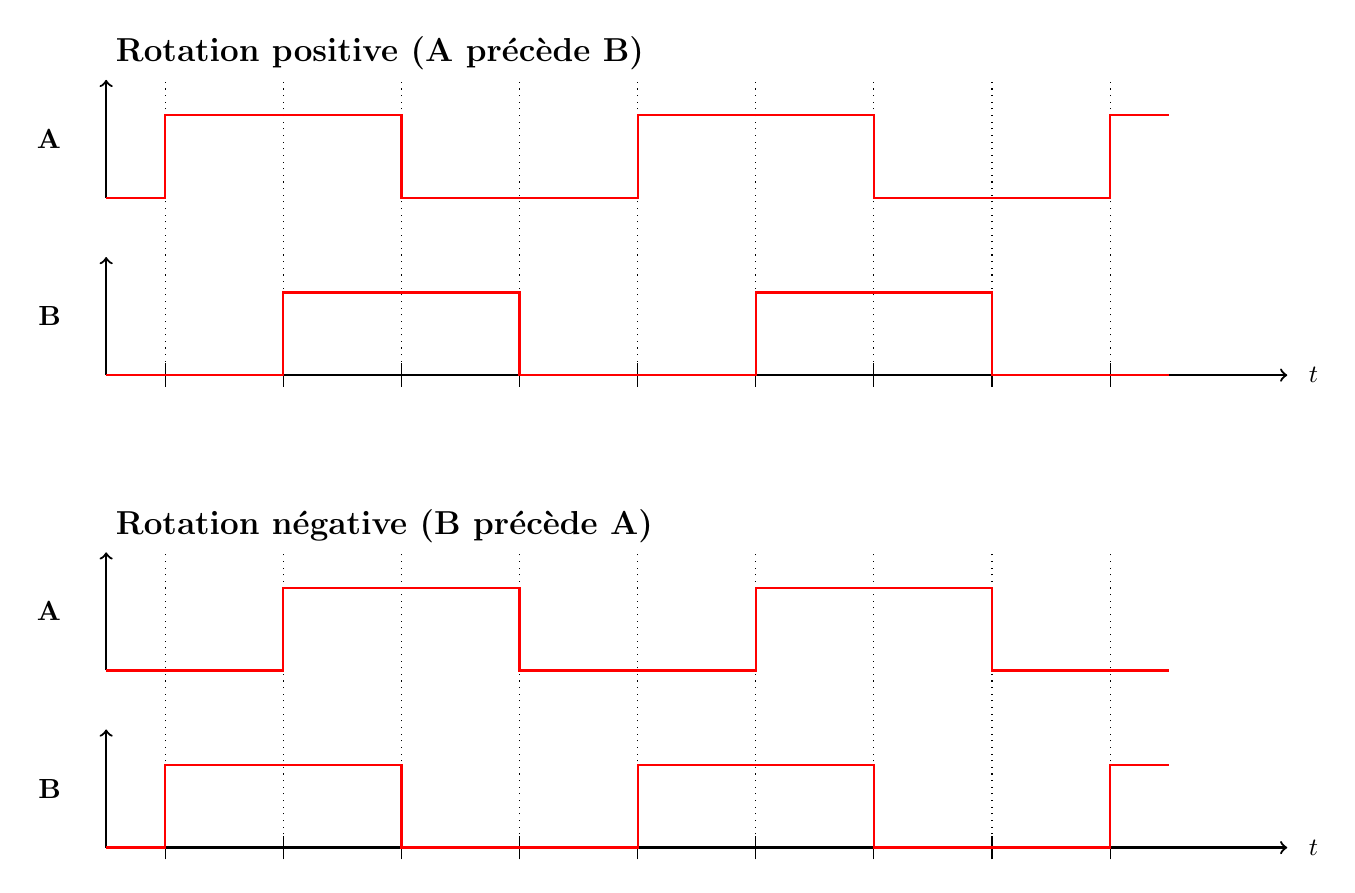
\begin{tikzpicture}[scale=1.5]
        % Titre Rotation positive
        \node[anchor=south west, font=\large\bfseries] at (0, 9) {Rotation positive (A précède B)};
        
        % Axe vertical pour A
        \draw[->, thick, black] (0, 8) -- (0, 9);
        \node[anchor=east] at (-0.3, 8.5) {\textbf{A}};
        
        % Axe vertical pour B
        \draw[->, thick, black] (0, 6.5) -- (0, 7.5);
        \node[anchor=east] at (-0.3, 7) {\textbf{B}};
        
        % Axe temps horizontal en bas
        \draw[->, thick, black] (0, 6.5) -- (10, 6.5);
        \node[anchor=west, font=\small] at (10.1, 6.5) {$t$};
        % Graduations et labels - alignées avec les fronts
        \draw[black] (0.5, 6.4) -- (0.5, 6.6);
        \draw[black] (1.5, 6.4) -- (1.5, 6.6);
        \draw[black] (2.5, 6.4) -- (2.5, 6.6);
        \draw[black] (3.5, 6.4) -- (3.5, 6.6);
        \draw[black] (4.5, 6.4) -- (4.5, 6.6);
        \draw[black] (5.5, 6.4) -- (5.5, 6.6);
        \draw[black] (6.5, 6.4) -- (6.5, 6.6);
        \draw[black] (7.5, 6.4) -- (7.5, 6.6);
        \draw[black] (8.5, 6.4) -- (8.5, 6.6);
        
        % Pointillés verticaux à chaque graduation
        \draw[dotted, thin, black] (0.5, 6.5) -- (0.5, 9);
        \draw[dotted, thin, black] (1.5, 6.5) -- (1.5, 9);
        \draw[dotted, thin, black] (2.5, 6.5) -- (2.5, 9);
        \draw[dotted, thin, black] (3.5, 6.5) -- (3.5, 9);
        \draw[dotted, thin, black] (4.5, 6.5) -- (4.5, 9);
        \draw[dotted, thin, black] (5.5, 6.5) -- (5.5, 9);
        \draw[dotted, thin, black] (6.5, 6.5) -- (6.5, 9);
        \draw[dotted, thin, black] (7.5, 6.5) -- (7.5, 9);
        \draw[dotted, thin, black] (8.5, 6.5) -- (8.5, 9);
        
        % Piste A - commence à 0 (en rouge) - premier front à t=0.5
        \draw[thick, red] (0, 8) -- (0.5, 8) -- (0.5, 8.7) -- (2.5, 8.7) -- (2.5, 8) -- (4.5, 8) -- (4.5, 8.7) -- (6.5, 8.7) -- (6.5, 8) -- (8.5, 8) -- (8.5, 8.7) -- (9, 8.7);
        
        % Piste B - commence à 0 (décalée de 1/4 de période, en rouge) - premier front à t=1.5
        \draw[thick, red] (0, 6.5) -- (1.5, 6.5) -- (1.5, 7.2) -- (3.5, 7.2) -- (3.5, 6.5) -- (5.5, 6.5) -- (5.5, 7.2) -- (7.5, 7.2) -- (7.5, 6.5) -- (9, 6.5);
        
        % Titre Rotation négative
        \node[anchor=south west, font=\large\bfseries] at (0, 5) {Rotation négative (B précède A)};
        
        % Axe vertical pour A
        \draw[->, thick, black] (0, 4) -- (0, 5);
        \node[anchor=east] at (-0.3, 4.5) {\textbf{A}};
        
        % Axe vertical pour B
        \draw[->, thick, black] (0, 2.5) -- (0, 3.5);
        \node[anchor=east] at (-0.3, 3) {\textbf{B}};
        
        % Axe temps horizontal en bas
        \draw[->, thick, black] (0, 2.5) -- (10, 2.5);
        \node[anchor=west, font=\small] at (10.1, 2.5) {$t$};
        % Graduations et labels - alignées avec les fronts
        \draw[black] (0.5, 2.4) -- (0.5, 2.6);
        \draw[black] (1.5, 2.4) -- (1.5, 2.6);
        \draw[black] (2.5, 2.4) -- (2.5, 2.6);
        \draw[black] (3.5, 2.4) -- (3.5, 2.6);
        \draw[black] (4.5, 2.4) -- (4.5, 2.6);
        \draw[black] (5.5, 2.4) -- (5.5, 2.6);
        \draw[black] (6.5, 2.4) -- (6.5, 2.6);
        \draw[black] (7.5, 2.4) -- (7.5, 2.6);
        \draw[black] (8.5, 2.4) -- (8.5, 2.6);
        
        % Pointillés verticaux à chaque graduation
        \draw[dotted, thin, black] (0.5, 2.5) -- (0.5, 5);
        \draw[dotted, thin, black] (1.5, 2.5) -- (1.5, 5);
        \draw[dotted, thin, black] (2.5, 2.5) -- (2.5, 5);
        \draw[dotted, thin, black] (3.5, 2.5) -- (3.5, 5);
        \draw[dotted, thin, black] (4.5, 2.5) -- (4.5, 5);
        \draw[dotted, thin, black] (5.5, 2.5) -- (5.5, 5);
        \draw[dotted, thin, black] (6.5, 2.5) -- (6.5, 5);
        \draw[dotted, thin, black] (7.5, 2.5) -- (7.5, 5);
        \draw[dotted, thin, black] (8.5, 2.5) -- (8.5, 5);
        
        \draw[thick, red] (0, 4) -- (1.5, 4) -- (1.5, 4.7) -- (3.5, 4.7) -- (3.5, 4) -- (5.5, 4) -- (5.5, 4.7) -- (7.5, 4.7) -- (7.5, 4) -- (9, 4);
        
        % Piste B - commence à 0 (B précède A, en rouge)
        \draw[thick, red] (0, 2.5) -- (0.5, 2.5) -- (0.5, 3.2) -- (2.5, 3.2) -- (2.5, 2.5) -- (4.5, 2.5) -- (4.5, 3.2) -- (6.5, 3.2) -- (6.5, 2.5) -- (8.5, 2.5) -- (8.5, 3.2) -- (9, 3.2);
        
    \end{tikzpicture}
    \caption{Chronogrammes selon le sens de rotation avec le codeur incrémental}
    \label{fig:chronogrammes_sens_rotation}
\end{figure}
